\clearpage\section{Chapter 18: Scanning and Parsing}

Scanners and parsers are language processing components routinely used
by writers of compilers and interpreters. Techniques developed for
scanning and parsing may be useful to any application that processes
complex input, such as:

\begin{itemize}
\item a desktop calculator with arithmetic expression evaluation
\item a \index{compiler}compiler for a programming language
\item an HTML style checker
\item a spreadsheet with formulas in the cells
\end{itemize}

This chapter describes versions of the classic UNIX scanner and parser
generators, \index{lex}\textsf{lex} and \index{yacc}\textsf{yacc}, that
support Unicon. The Unicon-friendly tools are called \textsf{ulex} and
\textsf{iyacc}. Note that scanning in this chapter refers to lexical
analysis as found in typical compilers, the processing of characters
one at a time to form words or tokens. This is not to be confused with
\ scanning an image of a piece of paper, nor is it synonymous with
Unicon{\textquotesingle}s built-in string scanning mechanism, although
string scanning can certainly be used to implement a scanner for a
compiler.

Building a \index{scanner}scanner or parser can be a daunting task for
the newcomer. However, if you start simple, it is very easy to work
with these very high-level tools with only a day{\textquotesingle}s
worth of experience. For people with experience using the C versions of
\textsf{lex} and \textsf{yacc}, be assured that the major features
available in those programs are supported here. Additional
documentation on \textsf{ulex} and \textsf{iyacc} are on the Unicon Web
page.

When you{\textquotesingle}re finished with this chapter, you will know
how to:

\begin{itemize}
\item \ build scanners using \textsf{ulex}
\item \ build parsers using \textsf{iyacc}
\item \ use the two tools together with Unicon{\textquotesingle}s data
structures
\item \ generate useful and appropriate syntax error messages using the
\textsf{merr} tool
\end{itemize}

\subsection{What are Scanning and Parsing?}

Scanning and parsing originate in the field of language recognition.
Consider the sentence \textit{This computer can run my software}.
Scanning is the recognition of words, the grouping of the characters
into contiguous blocks of letters such as \textit{This} and
\textit{computer}. \ The spaces are identified as separators
during scanning and ignored thereafter. The period that marks the end
of a sentence isn't a {\em word\/} in the traditional sense, but
such punctuation is identified in scanning and used in parsing to
mark the end of a sentence, after which it is no longer needed.

Parsing is the recognition of valid phrases and sentences. Most
sentences in English have a subject phrase and a verb phrase, and
optionally an object phrase. The rules that determine what is a valid
sentence form a {\em grammar\/}. Grammars go beyond telling whether
a sentence is syntactically correct or not, they help with sentence
understanding by indicating the organization and relationships between
words and phrases.

In the above sentence, \textit{This computer} is a
subject phrase, \textit{can run} is a verb phrase, and \textit{my
software} is an object phrase. In English, the modifier usually
comes before the 
thing modified within the phrases. So \textit{This} modifies
\textit{computer}, \textit{can} modifies \textit{run}, and \textit{my}
modifies \textit{software}. This hierarchical grouping of words is a
by-product of parsing. Figure 18-1 shows a parse \index{tree}tree for
the example sentence.


\bigskip

\begin{center}
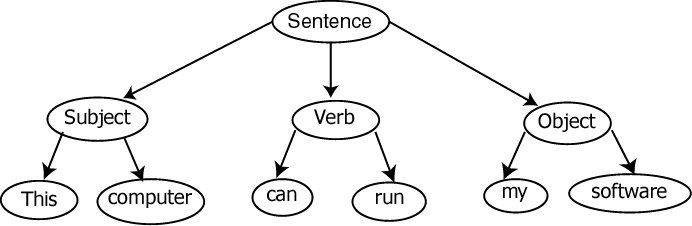
\includegraphics[width=5.4362in,height=1.7846in]{ub-img/ub-img64.png}
\end{center}

{\sffamily\bfseries Figure 18-1:}
{\sffamily Parse Tree for {\textquotedbl}This computer can run my
software{\textquotedbl}}

\bigskip

If you have studied linguistics, this description of scanning and
parsing may seem nauseatingly oversimplified, and if you have not, then
you may be lost already.  The study of human languages has shown them
to be quite complicated.  The tools presented in this chapter
don{\textquotesingle}t handle the complexities of human language, but
they use basic linguistic concepts to elegantly solve most problems
encountered in the processing of computer languages.

This chapter illustrates the use of \textsf{ulex} and
\textsf{iyacc} in Icon programs. It is not a comprehensive description
of these complex tools. If this chapter is your first introduction to
\textsf{lex} and \textsf{yacc}, you may wish to also read (Levine
1990), or consult a reference on writing compilers for more information
on these topics.

\subsection{ulex}

The name \textsf{ulex} stands for Unicon LEX. The \textsf{ulex}
program was written by Katie Ray with a little help from Clinton Jeffery
and is presently at an alpha-test stage of completion and maturity.
It is inspired by
the classic UNIX program called \textsf{lex} that dates back to 1975. The
\textsf{ulex} tool takes a lexical specification as input; the lexical
specification gives rules for forming words (and punctuation) to
be recognized.  For example a lexical specification might tell exactly
which characters are allowed in variable names, and exactly how the
various kinds of numeric constants are formed for a given language.
From this lexical specification, Ulex produces a lexical
analyzer (consisting of an Icon procedure) that corresponds to that
specification. A \index{lexical
analyzer}lexical analyzer is a fancy name for a scanner, and the
lexical analyzer generated by \textsf{ulex} is simply a procedure named
\textsf{yylex()}.

The rules that make up
\textsf{ulex} specifications consist of a list of {\em regular expressions\/}.
Chapter 3 described some library functions that employ \index{regular
expression} this notation for specifying the structure
of words. The specification of the lexical structure of many languages
can be concisely and precisely stated using this notation. You only
need to know the basics of regular expressions to use them productively.

\subsubsection{A Word Count Program}

There is a UNIX program called \textsf{wc}, short for \index{word
count}word count, that counts newlines, words, and characters in a
file. This section shows how to build such a program using
\textsf{ulex}. A short, albeit simplistic, definition of a word is any
sequence of non-white space characters. White space characters are
blanks and tabs. Listing 18-1 shows a complete \textsf{ulex} program that
operates like \textsf{wc}.  It can be compiled by the commands

\iconcode{
ulex wc.l
unicon wc
}

The first command translates from the lexical specification file wc.l
into a Unicon source file, wc.icn, which can then be compiled in the
usual way.

\pagebreak


\bigskip

{\sffamily\bfseries
Listing 18-1}

{\sffamily\bfseries
A simple word counter program, wc.l}

\iconcode{
ws \ \ \ [ {\textbackslash}t] \\
nonws [\^{} {\textbackslash}t{\textbackslash}n] \\
\ \\
\%\{ \\
global cc, wc, lc \\
\%\} \\
\ \\
\%\% \\
\ \\
\{nonws\}+ \> \> \> \> \{ cc +:= yyleng; wc +:= 1 \} \\
\{ws\}+ \> \> \> \> \{ cc +:= yyleng \} \\
{\textbackslash}n \> \> \> \> \{ lc +:= 1; cc +:= 1 \} \\
\ \\
\%\% \\
\ \\
procedure main() \\
\> cc := wc := lc := 0 \\
\> yylex() \\
\> write(right(lc, 8), right(wc, 8), right(cc, 8)) \\
end
}

All \textsf{ulex} programs, including this program, consist of three
sections, separated by lines containing two percent signs. The three
sections are the definitions section, the rules section, and the
procedures section.

In the word count program, the definitions section has two definitions,
one for white space (\textsf{ws}) and one for non-white space
(\textsf{nonws}). These definitions are followed by code to declare
three global variables, which will be used as counters. The variables
\textsf{cc}, \textsf{wc}, and \textsf{lc} are used to count the
characters, words, and lines, respectively.

The rules section in this example contains three rules. White space,
words, and newlines each have a rule that matches and counts their
occurrences. The rules each consist of a regular expression on the
left, followed by a {\em semantic action\/} consisting of Unicon code
in curly braces that executes when that regular expression is matched.

This \textsf{wc} code is a fine example, but a lot of the work
revolves around the trivial task of counting characters. You might
get a performance gain by deleting variable cc and the code that
computes it, and instead asking the system for the file size (possibly
using \textsf{where()} or \textsf{stat()}).

The procedure section has one procedure, \textsf{main()}. It calls the
lexical analyzer and then prints out the counts. There are many ways to
write this word count program, with different performance
characteristics. If speed is your primary consideration you can look in
the documentation for \textsf{flex} (Paxson 1995) to get five
progressively more complex but faster versions of word count.

\subsubsection{A Lexical Analyzer for a Desktop Calculator}

The above example illustrates using \textsf{ulex} to write standalone
programs, but the function \textsf{yylex()} produced by \textsf{ulex}
is usually called by a parser that does subsequent syntax checking
against a grammar. The \textsf{yylex()} function
can be used to produce a sequence of words, and a parser such as that
generated by the \textsf{iyacc} program determines how those words may
be combined into sentences, if possible. For this reason, it makes
sense to study how \textsf{ulex} is used in this typical context.

One primary difference between using ulex as a standalone tool and
using it to aid a parser is that in the earlier example,
\textsf{yylex()} was only called once to process an entire file. In
contrast, when a parser uses \textsf{yylex()} it calls it repeatedly,
and \textsf{yylex()} returns repeatedly, supplying the parser with each
word that it finds. You will see this in the following example.

A calculator program is simple enough to understand in one sitting and
complex enough to get a sense of how to use \textsf{ulex} with its
parser generator counterpart, \textsf{iyacc}. In general, in a desktop
calculator program, the user types in complex formulas and the
calculator evaluates them and prints out the answer.  The lexical
analyzer helps convert the string of characters that are input into
the numbers and operators to be evaluated.  The parser enforce the
operator precedence rules and check for correctness; it will be shown
later during the discussion of iycc.

First things first: what are the \textit{words} of this little language?
Numbers, math operators, and variable names. A number is one or more
digits followed by an optional decimal point and one or more digits. In
regular expressions, you can write this as

\iconcode{
[0-9]+({\textbackslash}.[0-9]*)?
}

The 0 through 9 is specified with a range using a dash for characters
within the square brackets. The plus sign means one or more
occurrences, whereas the star means \textit{zero} or more occurrences.
The backslash period means literally match a period; without a
backslash a period matches any single character. \ The parentheses are
used for grouping and the question mark means zero or more times.

The math operators are simple {\textquotedbl}words{\textquotedbl}
composed of one character such as the plus sign, minus sign, and star
for multiplication. Variable names need to be meaningful; so why not
let them be any combination of letters, digits, and underscores. You do
not want to confuse them with numbers, so refine the definition by
making sure that variables do not begin with a number. This definition
of variable names corresponds to the following regular expression: 

\iconcode{
[a-zA-Z\_][a-zA-Z0-9\_]*}

Here is some more information about the three sections that make up an
\textsf{ulex} program. The definitions section contains Unicon code
that is copied verbatim into the generated final program, before the
generated scanner code. You can put \textsf{\$include} statements there
to define symbolic constants for the different kinds of words in your
scanner. The rules section contains a series of rules, composed of two
parts: a regular expression and a fragment of Unicon code that executes
whenever that regular expression matches part of the input. The
procedures section contains arbitrary code that is copied verbatim
after the generated scanner{\textquotesingle}s code. A complete scanner
specification for the desktop calculator looks like:

\iconcode{
\%\{ \\
\# y\_tab.icn contains the symbol definitions for integer values \\
\# representing the terminal symbols NAME, NUMBER, and \\
\# \index{assignment}ASSIGNMENT. It is generated with iyacc \textrm{$-$}d calc.y \\
\$include y\_tab.icn \\
\%\} \\
\ \\
letter \ \ \ \ [a-zA-Z\_] \\
digiletter [a-zA-Z0-9\_] \\
\ \\
\%\% \\
\ \\
\{letter\}\{digiletter\}* \> \> \> \> \> \> \> \{ yylval := yytext; return NAME \} \\
$[0-9]+$
({\textbackslash}.[0-9]+)? \> \> \> \> \> \> \> \{ yylval := numeric(yytext);
return NUMBER \} \\
{\textbackslash}n \> \> \> \> \> \> \> \{ return 0 \} \\
{\textquotedbl}:={\textquotedbl}
\> \> \> \> \> \> \> \{ return ASSIGNMENT \} \\
$[$ {\textbackslash}t$]+$ \\
 .\> \> \> \> \> \> \> \{ return ord(yytext) \} \\
\%\%
}

There are a couple of details about \textsf{ulex} and \textsf{iyacc}
worth noting in this scanner. The \textsf{ulex} tool maintains a global
variable named \textsf{yytext} that holds the characters that match a
given regular expression. For example, a plus operator is returned by
the scanner rule that says to return the character code corresponding
to \textsf{yytext}, \textsf{ord(yytext)}, on the regular expression
that consists of a lone period (\texttt{.} matches any one character).

Even if \textsf{yytext} is not part of
\textsf{yylex()}{\textquotesingle}s return value for a token, there are
situations in which the string is of interest to the parser, which
reads lexical values from a global variable called \textsf{yylval}.
When a variable name is encountered, it makes sense to copy
\textsf{yytext} over into \textsf{yylval}. On the other hand, when a
number is encountered, the numeric value corresponding to the
characters in \textsf{yytext} is computed and stored in
\textsf{yylval}. Since Icon allows a variable to hold any type of
value, there is no need for a union or some other messy construct to
handle the fact that different tokens have different kinds of lexical
values.

\subsubsection{A Summary of the Regular Expression Operators:}

The above example only uses a few of the regular expression operators.
Table 18-1 lists the most commonly used operators in \textsf{ulex}.
Advanced users will want to consult the documentation for \textsf{flex}
or its predecessor, \textsf{lex}, for a more complete list.

\vspace{0.16in}

{\centering\sffamily\bfseries
Table 18-1
\par}

{\centering\sffamily\bfseries
Commonly used lex operators
\par}

\vspace{-0.10in}
\begin{flushleft}
\begin{supertabular}{|m{0.7268598in}|m{5.1156597in}|}
\hline
\sffamily\bfseries Operator &
\sffamily\bfseries Description\\\hline
. &
Matches any single character except the newline character.\\\hline
* &
Matches zero or more occurrences of the preceding expression.\\\hline
[] &
This is a character class that matches any character within the
brackets. \ If the first character is a caret (\^{}), then it changes
the meaning to match any character \textit{except} those within the
brackets. \ A dash inside the brackets represents a character range, so
[0-9] is equivalent to [0123456789]. \ \\\hline
\^{} &
Matches the beginning of a line. This interpretation is used only when
the caret is the first character of a regular expression.\\\hline
\$ &
Matches the end of a line. This interpretation is used only when the
dollar symbol is the last character of a regular expression.\\\hline
{\textbackslash} &
Used to escape the special meaning of a character. For example,
{\textbackslash}\$ matches the dollar sign, not the end of a
line.\\\hline
+ &
Matches one or more occurrences of the preceding expression. For
example, [0-9]+ matches {\textquotedbl}1234{\textquotedbl} or
{\textquotedbl}734{\textquotedbl} but not the empty string.\\\hline
? &
Matches zero or more occurrences of the preceding expression. For
example, -?[0-9]+ matches a number with an optional leading negative
sign.\\\hline
{\textbar} &
Matches either the preceding regular expression or the one following it.
So Mar{\textbar}Apr{\textbar}May matches any one of these three
months.\\\hline
{\textquotedbl}...{\textquotedbl} &
Matches everything in quotes literally.\\\hline
() &
Groups a regular expression together, overriding the default operator
precedence. This is useful for creating more complex expressions with
*, +, and {\textbar}.\\\hline
\end{supertabular}
\end{flushleft}
Before you conclude your study of \textsf{ulex}, two subtle points are
worth knowing. The matches allowed by a list of regular expressions are
often ambiguous, and this is normal and healthy. For example, does
\textsf{count10} match a variable name and then an integer, or just one
variable name? The \textsf{ulex} tool matches the longest substring of
input that can match the regular expression. So it matches
\textsf{count10} as one word, which is a variable name in this case.
There is one more sticky point: what if two rules match the exact same
input characters, with no longest match to break the tie? In this case,
\textsf{ulex} picks the first rule listed in the specification that
matches, so the order of the rules can be important.

\subsubsection{Lexical analyzers in real compilers}
Lexical analyzers in real compilers will exhibit some differences from
the desktop calculator example. For one thing, more than half of the
compilers out there use handwritten lexical analyzers instead of
lex-generated ones. This is because lexical analyzer speed is
significant to overall compilation speed, and because not every
behavior needed in lexical analyzers is easily handled by regular
expressions. Nevertheless, ulex might save a lot of programmer time,
both in the initial development and in the later maintenance phase when
changes are needed. Here are some more practical tips when using ulex.

\liststyleLvii
\begin{itemize}
\item Define a record type to hold lexical attributes. Depending on your
language, this may consist only of filename, and line number for error
reports, or it might involve useful computation, such as de-escaping
literal strings, or computing integer values from octal or hexadecimal
constants. For each token, allocate a new record instance and assign
\textsf{yylval} to refer to it.
\item Your lexical analyzer code may be smaller if you place reserved
words in a table, and look them up after matching the pattern for
variable names, instead of writing a separate regular expression for
each reserved word. If you \textit{do} choose to write separate regular
expressions for each reserved word, remember to put them
\textit{before} the rule for variable names, or your reserved word
patterns will never be used.
\item Keep your integer codes consistent between your scanner and your
parser, or you will get nonsense errors that are hard to debug. This
tends to happen when you add or change the integer codes for symbolic
token names. At such times it is important to recompile both scanner
and parser to maintain their consistency.
\end{itemize}
\subsection{iyacc}
The name \textsf{iyacc} stands for Icon YACC. It is a variant of a
program called \textsf{byacc} (Berkeley \index{yacc}YACC), modified to
generate Icon code as an alternative to C. Berkeley YACC in turn is a
public domain replacement for the original AT\&T YACC, which stands for
Yet Another Compiler Compiler. The \textsf{iyacc} program takes a
\index{context-free grammar}\index{grammar}grammar that you specify and
generates a parser that recognizes correct sentences. A parser allows
you to do more than just tell whether a sentence is valid according to
the grammar, it allows you to record the structure of the sentence for
later use. This internal structure explains \textit{why} the sentence
is grammatical, and it is also the starting point for most translation
tasks. The structure is often a tree called a \index{parse
tree}\textit{parse }\index{tree}\textit{tree}.

The language used by \textsf{iyacc} to express the grammar is based on a
form of \index{BNF}BNF, which stands for \index{Backus-Naur
Form}Backus-Naur Form. A grammar in BNF consists of a series of
production rules, each one specifying how a component of the parse is
constructed from simpler parts. For example, here is a grammar similar
to the one used to build the calculator:

\iconcode{
\index{assignment}assignment : NAME := expression \\
expression : NUMBER \\
\>   \ \ \ \ \ \ \ \ {\textbar} expression + NUMBER \\
\>   \ \ \ \ \ \ \ \ {\textbar} expression \textrm{$-$} NUMBER
}

This grammar has two rules. The symbol to the left of the colon is
called a \textit{non-terminal} symbol. This means that the symbol is an
abstraction for a larger set of symbols. Each symbol to the right of
the colon can be either another non-terminal or a \textit{terminal}
symbol. If it is a terminal, then the scanner will recognize the
symbol. If it is not, then a rule will be used to match that
non-terminal. It is not legal to write a rule with a terminal to the
left of the colon. The vertical bar means there are different possible
matches for the same non-terminal. For example, an expression can be a
number, an expression plus a number, or an expression minus a number.

As was mentioned previously, the most common way to represent the result
of parsing is a tree. For example, if the input string is
\textsf{{\textquotedbl}count := 10 + 99{\textquotedbl}}, then the parse
tree for the above grammar would look like Figure 18-2. Note how the
terminal symbols NAME and NUMBER have lexical attribute values provided
by the scanner.


\bigskip

\begin{center}
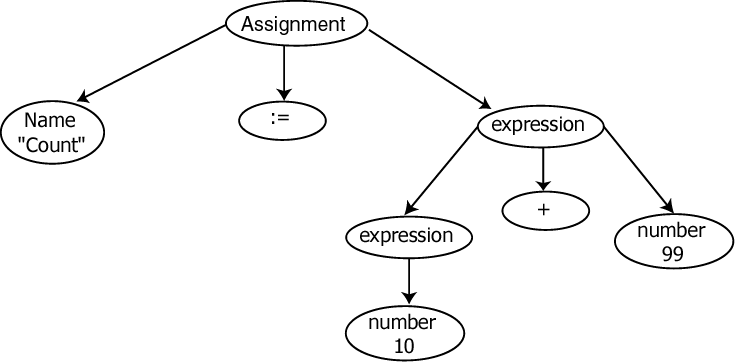
\includegraphics[width=5.8752in,height=2.8929in]{ub-img/ub-img65.png}
\end{center}

{\sffamily\bfseries Figure 18-2:}
{\sffamily Parse Tree for {\textquotedbl}count := 10 + 99{\textquotedbl}}

\bigskip

The \textsf{iyacc} program{\textquotesingle}s input files are structured
much like \textsf{ulex}{\textquotesingle}s input files. They have a
definitions section, a rules section, and a procedures section. The
definitions section includes code to be copied into the output file
before the parser code, surrounded by \textsf{\%\{} and \textsf{\%\}}.
This section also includes the declarations of each of the
\textit{tokens} that are going to be returned by the scanner. The term
{\textquotedbl}token{\textquotedbl} is just another name for a terminal
symbol, or a word. Tokens can be given a left or right associativity,
and they are declared from lowest precedence to highest precedence. You
may want to consult a reference on \texttt{yacc} for details on how
these features are used.

The next section is the rules section. The left and right sides of a
rule are separated by a colon. The right side of the rule can be
embedded with semantic actions consisting of Unicon code that is
surrounded by curly braces. The last section is the procedures section.

When the parser matches a rule, it executes the Unicon code for the
semantic action associated with the rule, if there is any. Actions can
appear anywhere on the right-hand side of a rule, but their semantics
are intuitive only at the end a rule. Vertical bars actually mark
alternative rules, so it makes sense to have a (possibly different)
action for each alternative. The action code may refer to the value of
the symbols on the right side of the rule via the special variables
\textsf{\$1}, \textsf{\$2}... and they can set the value of the symbol
on the left of the colon by assigning to the variable \textsf{\$\$}.
The value of a terminal symbol is the contents of variable
\textsf{yylval}, which is assigned by the scanner. The value of a
non-terminal is the value assigned to the \textsf{\$\$} variable in the
grammar rule that produced that non-terminal. As was mentioned for the
\textsf{yylval} variable, in other languages, assigning different kinds
of values to \textsf{\$\$} for different non-terminals is awkward. In
Unicon, it is very easy because variables can hold values of any type.

\subsubsection{Parse Tree Construction}
The Unicon translator itself provides a classic demonstration of parse
tree construction using \textsf{iyacc}. The Unicon grammar lives in
\textsf{uni/unicon/unigram.y} in the Unicon distributions. Semantic
actions within that grammar build a parse tree using a record type
\textsf{treenode} and a variable argument function constructor:

\iconcode{
record treenode(label, children) \\
procedure node(label, children[]) \\
\>   return treenode(label, children) \\
end
}

This sneaky listification could be avoided if Unicon were extended to
support variable-argument record constructors! In any case, the iyacc
semantic actions that build typical parse tree nodes look like:

\iconcode{
expr6: expr6 PLUS expr7 \{ \$\$ :=
node({\textquotedbl}Bplus{\textquotedbl}, \$1, \$2, \$3) \}}

Note that the label is not just
{\textquotedblleft}plus{\textquotedblright} because there are two
{\textquotedblleft}plus{\textquotedblright} operators, unary and
binary, hence the {\textquotedblleft}Bplus{\textquotedblright} to
denote binary addition. No tree construction example would be complete
without the basis case in which leaves are constructed. As is mentioned
above, leaves such as the \textsf{PLUS} token in the rule given above
are constructed by the lexical analyzer and passed to the parser in the
global variable \textsf{yylval}. Tokens are records with the
declaration:

\iconcode{
record token(tok, s, line, column, filename)}

\noindent
where \textsf{tok} is the token{\textquotesingle}s integer code,
\textsf{s} is its string lexeme, and \textsf{line}, \textsf{column},
and \textsf{filename} are attributes that record its source code
location for error reporting and debugging purposes. It is this type of
value, provided by the lexical analyzer, that is sitting in
\textsf{\$2} at the time \textsf{node()} is called to produce the
internal tree node for \textsf{expr6}.

\subsubsection{A Syntax Analyzer for a Desktop Calculator}
Returning to our desktop calculator example, in the calculator, there is
one procedure, \textsf{main()}, that calls the parser once for each
line. Listing 18-2 shows a complete parser for the desktop calculator.

\bigskip

{\sffamily\bfseries
Listing 18-2}

{\sffamily\bfseries
The desktop calculator in calc.y}

\iconcode{
\%\{ \\
\#\# add any special linking stuff here \\
global vars \\
\%\} \\
\ \\
/* YACC Declarations */ \\
\%token NUM, NAME, ASSIGNMENT \\
\%left {\textquotesingle}-{\textquotesingle}
{\textquotesingle}+{\textquotesingle} \\
\%left {\textquotesingle}*{\textquotesingle}
{\textquotesingle}/{\textquotesingle} \\
\%left NEG \ \ \ \ /* negation-{}-unary minus */ \\
\%right {\textquotesingle}\^{}{\textquotesingle} \ \ \ /* exponentiation
\ \ \ \ \ \ \ */ \\
\ \\
/* Grammar follows */ \\
\%\% \\
input: \ \ \ /* empty string */ \\
\>   \ \ {\textbar} input line \\
\>   \ \ ; \\
\ \\
line: \ \ \ \ {\textquotesingle}{\textbackslash}n{\textquotesingle} \\
\>   \ {\textbar} exp
{\textquotesingle}{\textbackslash}n{\textquotesingle} \ \{ write(\$1)
\} \\
\>   \ {\textbar} NAME ASSIGNMENT exp
{\textasciigrave}{\textbackslash}n{\textquotesingle} \{  \\
\>   \ \ \ \ \ \ vars[\$1] := \$3  \\
\>   \ \ \ \ \ \ write(\$3) \\
\>   \ \ \ \ \ \ \} \\
\>   \ ; \\
\ \\
exp: NUM \ \ \ \ \ \ \ \ \ \ \ \ \ \ \ \ \ \{ \$\$ := \$1
\ \ \ \ \ \ \} \\
\>   {\textbar} NAME \ \ \ \ \ \ \ \ \ \ \ \ \ \ \{ \$\$ := vars[\$1]
\} \\
\>   {\textbar} exp {\textquotesingle}+{\textquotesingle} exp
\ \ \ \ \ \ \ \{ \$\$ := \$1 + \$3 \ \} \\
\>   {\textbar} exp {\textquotesingle}-{\textquotesingle} exp
\ \ \ \ \ \ \ \{ \$\$ := \$1 - \$3 \ \} \\
\>   {\textbar} exp {\textquotesingle}*{\textquotesingle} exp
\ \ \ \ \ \ \ \{ \$\$ := \$1 * \$3 \ \} \\
\>   {\textbar} exp {\textquotesingle}/{\textquotesingle} exp
\ \ \ \ \ \ \ \{ \$\$ := \$1 / \$3 \ \} \\
\>   {\textbar} {\textquotesingle}-{\textquotesingle} exp \ \%prec NEG
\{ \$\$ := -\$2 \ \ \ \ \ \} \\
\>   {\textbar} exp {\textquotesingle}\^{}{\textquotesingle} exp
\ \ \ \ \ \ \ \{ \$\$ := \$1 \^{} \$3 \ \} \\
\>   {\textbar} {\textquotesingle}({\textquotesingle} exp
{\textquotesingle}){\textquotesingle} \ \ \ \ \ \ \ \{ \$\$ := \$2
\ \ \ \ \ \ \} \\
\>   ; \\
\%\% \\
\ \\
procedure main() \\
\>   vars := table(0) \# initialize all variables to zero \\
\>   write({\textquotedbl}iyacc Calculator Demo{\textquotedbl}) \\
\ \\
\>   repeat \{ \\
\>   \ \ write({\textquotedbl}expression:{\textquotedbl})  \\
\>   \ \ yyparse() \\
\>   \} \\
end
}

You can use single quoted characters as tokens without declaring them,
so \textsf{{\textquotesingle}+{\textquotesingle}},
\textsf{{\textquotesingle}-{\textquotesingle}},
\textsf{{\textquotesingle}*{\textquotesingle}},
\textsf{{\textquotesingle}/{\textquotesingle}},
\textsf{{\textquotesingle}\^{}{\textquotesingle}},
\textsf{{\textquotesingle}({\textquotesingle}}\texttt{,
}\textsf{{\textquotesingle}){\textquotesingle}} are not declared in the
above grammar. The unary minus makes use of the \textsf{\%prec} keyword
to give it priority over binary minus. Note that these are
\textsf{yacc} notation for small integers;
\textsf{{\textquotesingle}+{\textquotesingle}} is a shorthand for
\textsf{ord({\textquotedbl}+{\textquotedbl})} here, not a cset. Tokens
NUM, NAME, ASSIGNMENT, and NEG are declared.

\subsubsection{Making It All Work From The Command-Line}
How do you combine all these tools correctly to build a program? Here is
the sequence of commands you would type for creating a calculator given
the ulex and iyacc input files presented earlier. You might normally
use a {\textquotedbl}make{\textquotedbl} program that manages the
dependencies of different files and programs, to avoid typing this all
by hand, but {\textquotedbl}make{\textquotedbl} is beyond the scope of
this chapter.


\bigskip

\iconcode{
\$ iyacc \textrm{$-$}d calc.y\ \ \ \ \ \ c\textit{reates calc.icn \&
y\_tab.icn} \\
\$ ulex calc\_lex.l \ \ \ \ \ \ \textit{creates calc\_lex.icn} \\
\$ unicon calc.icn calc\_lex.icn \ \ \textit{creates the program calc}
}

The resulting calculator program might be executed in a session such as
the following:

\iconcode{
\$ calc \ \ \ \ \ \ \ \ \ \ \ \ \ \ \ \ \ \ \ \textit{runs calc} \\
iyacc Calculator Demo \\
expression: (3 + 5)*2 \ \ \ \ \textit{enter an expression} \\
16 \ \ \ \ \ \ \ \ \ \ \ \ \ \ \ \ \ \ \ \ \ \ \ \textit{prints out the
answer} \\
expression: x := 16 \ \ \ \ \ \ \textit{enter an expression} \\
16 \ \ \ \ \ \ \ \ \ \ \ \ \ \ \ \ \ \ \ \ \ \ \ \textit{prints out the
answer} \\
expression: 2 * x \ \ \ \ \ \ \ \ \textit{enter an expression} \\
32 \ \ \ \ \ \ \ \ \ \ \ \ \ \ \ \ \ \ \ \ \ \ \ \textit{prints out the
answer} \\
expression: \^{}D \ \ \ \ \ \ \ \ \ \ \ control-D stop the program
}

\subsection[Generating Syntax Error Messages with Merr]{Generating
Syntax Error Messages with Merr}

\index{merr}When a syntax error occurs, iyacc-generated parsers call a
user-defined procedure named \textsf{yyerror(s)}; which by default
writes out \textsf{s}. Usually, the string passed into
\textsf{yyerror()} is {\textquotedbl}parse error{\textquotedbl} or
{\textquotedbl}syntax error{\textquotedbl}; not very helpful to the
unlucky person who has to fix the problem. If you write your own
\textsf{yyerror()} function, you can improve this error message by
including lexical information such as filename, line number, and the
token on which the error was detected; this is all expert programmers
usually need.

Those mortals who dare to program can use all the help you can give them
in interpreting their errors.\textit{ Merr} is a\textit{ }unique tool
you can use to produce better syntax error messages from your YACC
parsers. Merr was originally developed for the Unicon translator, but
is easily used in other YACC applications; it is included in the
uni/unicon directory in Unicon distributions.

\subsubsection{Merr Error Specification Files}
To use Merr, you give it a file named \textsf{meta.err} that contains a
set of example errors, along with an appropriate message for each
error. For example:

\iconcode{
int main\{\} ::: parenthesis or semi-colon expected \\
int x y; ::: missing comma in variable list \\
char () \{ \} ::: function name expected \\
int a[] = \{1,2; ::: unclosed initializer \\
struct foo int x; ::: missing \{ after struct label
}

In each case, \textsf{:::} is used to separate the error fragment from
the diagnostic message; error examples can span multiple lines when it
will help. Merr will run your compiler separately on each error to
figure out the corresponding parse state and token, and then generate a
yyerror() function that writes the error messages when those parse
state and input token combinations are seen by the parser.

\subsubsection{The Merr Command Line}

Merr is invoked from the directory in which your compiler is built, with
the following command line arguments and options:

\iconcode{
merr [-yYB] [-s make] [-o msgfile] \textit{compiler} [\textit{target}]}

\noindent
where \textit{compiler} is the name of the compiler for whom error
messages will be generated, and \textit{target} is the source filename
that the errant programs will be written to and compiled from,
defaulting to \textsf{m\_err.icn} (or \textsf{m\_err.c}). Merr executes
a system command to rebuild the compiler in order to create its error
message table. The default command is

\iconcode{
make \textit{compiler}}

The \textsf{{}-s} option overrides this default, as in the line

\iconcode{
merr -s {\textquotedblleft}make all{\textquotedblright} mycc bug.c}

Merr writes the error message table and \textsf{yyerror()} function to a
file named \textsf{yyerror.icn} (or \textsf{yyerror.c}) by default. The
\textsf{{}-o} option directs Merr to write the file with a different
name. Command line options \textsf{{}-y}, \textsf{{}-Y}, and
\textsf{{}-B} direct Merr to generate compatible C \textsf{yyerror()}
functions for Berkeley YACC, AT\&T YACC, and Bison, respectively. For
AT\&T YACC and Bison, Merr writes a header file \textsf{yyerror.h} that
defines a macro to add the parse state information to the yyerror()
function; this header file must be included in the YACC specification
(.y) file.

\subsection{Final Tips For Using ulex and iyacc}

Tasks requiring the processing of languages with a computer program can
vary greatly in complexity from very simple to extremely complex. As
the complexity grows, \textsf{ulex} and \textsf{iyacc} are two tools
that can make the scanning and parsing part of the task very easy to
manage. Because each tool makes the grammar of the language they are
processing very explicit in the code, programs written with these tools
are often easier to maintain than programs with handwritten scanners
and parsers. Each tool can be used independently and they also work
well together. Adding a little language to your application can make it
a more powerful and general tool. Imagine how much less useful
spreadsheets would be if you could not enter formulas in the cells.
Those formulas are a little language!

Since Unicon already has high-level string processing facilities, it is
worth asking how \textsf{ulex} and \textsf{iyacc} relate to the
language, or why they are needed. One answer is that they are standard
tools expected by \index{compiler}compiler writers. Another answer is
that they use special-purpose notations and algorithms to deliver
higher performance than is provided by Unicon{\textquotesingle}s more
general and more flexible facilities, and they do this from simpler
specifications. A final answer is that these tools are not mutually
exclusive of Unicon{\textquotesingle}s other features and you should
use whatever combination of these tools and Icon{\textquotesingle}s
built-in facilities are appropriate to the task at hand.

\subsection{Summary}

This chapter only scratches the surface of the features provided by
u\textsf{lex} and \textsf{iyacc}. \ The goal is to introduce you to the
capabilities of these tools that are now easy to use with Icon. In
fact, in many ways it is much easier to use these tools with Icon than
it is to use them with C, thanks to Icon{\textquotesingle}s string
processing facilities and built-in data structures. 

\clearpage
\bigskip

